\documentclass[conference]{IEEEtran}
\usepackage{times}
\usepackage[numbers]{natbib}
\usepackage{multicol}

% Constants for the RSS paper (rss/*.tex).
% The "corl" prefix is kept from the CoRL version of this paper.
%
% Source of truth: gaitnet-docs/ (methodology.md, training-setup.md,
% experiment-setup.md, results.md, runs.md), state of 2026-10-13. Each block
% names the file and section it comes from. The policy is SC-idm@1590
% (inverse footstep model in the loop). The paper calls the method GaitNet;
% gaitnet-docs calls the same network GaitNet-T.
%
% Convention: every macro below holds a bare value (a number, or a short
% math expression like 10^{-3}) with NO unit, %, or $ baked in. Units,
% percent signs, and math-mode delimiters are added at the call site, so a
% macro can be dropped into either running text or an equation unchanged.
% Numbers that appear only inside one table are written in that table, with
% a comment naming the eval they come from.

% --- Rates and action timing (methodology.md 1-2, README conventions) ---
\newcommand{\corlPhysicsHz}{250}
\newcommand{\corlControlHz}{25}
\newcommand{\corlControlTickMs}{40}
\newcommand{\corlMpcHz}{50}
\newcommand{\corlSwingDurationMin}{0.1}
\newcommand{\corlSwingDurationMax}{0.3}
\newcommand{\corlMinTicksPerSwing}{3}
\newcommand{\corlMaxTicksPerSwing}{8}
\newcommand{\corlMaxConcurrentSwingLegs}{2}
\newcommand{\corlMinContactLegs}{3}

% --- Footstep candidates (methodology.md 3) ---
\newcommand{\corlScanRays}{41}
\newcommand{\corlScanResCm}{1}
\newcommand{\corlPoolKernel}{5}
\newcommand{\corlGridCells}{37}
\newcommand{\corlGridReachCm}{18}
\newcommand{\corlMarginCm}{2}
\newcommand{\corlHipDropMax}{0.5}
\newcommand{\corlNumLegs}{4}
\newcommand{\corlTrainCandidatesPerLeg}{16}
\newcommand{\corlTotalCandidates}{65}

% --- Observation (methodology.md 4) ---
\newcommand{\corlStateDim}{25}
\newcommand{\corlFootPosDim}{8}
\newcommand{\corlVelDim}{3}
\newcommand{\corlAngVelDim}{3}
\newcommand{\corlGravityDim}{3}
\newcommand{\corlContactDim}{4}
\newcommand{\corlCandFeatDim}{8}
\newcommand{\corlHistTicks}{25}
\newcommand{\corlHistFeatDim}{26}
\newcommand{\corlHistSeconds}{1}
\newcommand{\corlObsDim}{1195}

% --- Networks (methodology.md 5) ---
\newcommand{\corlStateEncoderLayers}{3}
\newcommand{\corlStateEncoderHidden}{128}
\newcommand{\corlFootstepEncoderLayers}{2}
\newcommand{\corlFootstepEncoderHidden}{64}
\newcommand{\corlTrunkLayers}{3}
\newcommand{\corlMixerLayers}{2}
\newcommand{\corlMixerDim}{128}
\newcommand{\corlMixerHeads}{4}
\newcommand{\corlMixerFF}{256}
\newcommand{\corlParamsPerCandidateK}{99}   % thousands of parameters
\newcommand{\corlParamsGaitNetK}{464} % thousands of parameters
\newcommand{\corlDurationExploreStd}{0.01}

% --- Training controller (methodology.md 2) ---
\newcommand{\corlMpcHorizonSteps}{10}
\newcommand{\corlMpcHorizon}{0.2}
\newcommand{\corlFrictionMu}{0.8}
\newcommand{\corlAdmmIters}{80}
\newcommand{\corlGpuTorqueErrMax}{0.20}
\newcommand{\corlGpuTorqueErrPct}{0.6}
% Landing overshoot along the walking direction, training controller, no
% IDM (results.md 2; DEC 2026-10-12 17:30). Centimetres.
\newcommand{\corlOvershootSlowMin}{1.3}
\newcommand{\corlOvershootSlowMax}{1.9}
\newcommand{\corlOvershootFastMin}{2.9}
\newcommand{\corlOvershootFastMax}{3.9}

% --- Inverse footstep model (methodology.md 6) ---
\newcommand{\corlIdmInputDim}{33}
\newcommand{\corlIdmHidden}{256}
\newcommand{\corlIdmFootsteps}{180{,}681}
\newcommand{\corlIdmPerturbCm}{3}
\newcommand{\corlIdmHeldOutPct}{10}
\newcommand{\corlIdmRmsCm}{0.89}
\newcommand{\corlIdmIdentityRmsCm}{2.61}

% --- Training (training-setup.md 2-12) ---
\newcommand{\corlParallelEnvs}{1024}
\newcommand{\corlRolloutSteps}{100}
\newcommand{\corlPpoEpochs}{8}
\newcommand{\corlMiniBatches}{8}
\newcommand{\corlLearningRate}{3 \times 10^{-4}}
\newcommand{\corlClip}{0.3}
\newcommand{\corlEntropyCoef}{0.02}
\newcommand{\corlGamma}{0.99}
\newcommand{\corlLambda}{0.95}
\newcommand{\corlEpisodeSeconds}{20}
\newcommand{\corlAliveWeight}{0.4}
\newcommand{\corlTrackXyStd}{0.1}
\newcommand{\corlTrackYawStd}{0.2}
\newcommand{\corlActionPenalty}{0.4}      % magnitude; the sign is in the reward equation
\newcommand{\corlTerminationPenalty}{200} % magnitude; the sign is in the reward equation
\newcommand{\corlTiltLimitDeg}{20}
\newcommand{\corlMinBaseHeight}{0.15}
\newcommand{\corlFootDepthLimit}{0.05}
\newcommand{\corlCmdVxMax}{0.2}
\newcommand{\corlCmdYawMax}{0.2}
\newcommand{\corlTerrainCellCm}{12.5}
\newcommand{\corlVoidDepth}{0.5}
\newcommand{\corlTileSize}{4}
\newcommand{\corlNumLevels}{12}
% Author, 2026-10-14: the deployed run (SC-idm@1000) trained on 0-40 %
% voids; gaitnet-docs' 0-50 % is the curriculum's nominal top level.
\newcommand{\corlMaxVoidPct}{40}
\newcommand{\corlCurriculumProgress}{0.3}
\newcommand{\corlWalkPUp}{0.1}
\newcommand{\corlWalkPDown}{0.3}
\newcommand{\corlWalkRandomPct}{25}
% Step-recipe controller randomisation (training-setup.md 8).
\newcommand{\corlRandTrackMin}{0.3}
\newcommand{\corlRandPlanarMin}{0.5}
\newcommand{\corlRandApexMin}{0.07}
\newcommand{\corlRandApexMax}{0.12}
\newcommand{\corlRandBiasCm}{2}
\newcommand{\corlRandNoiseCm}{1}
% History of the deployed checkpoint (runs.md, training-setup.md 11).
\newcommand{\corlTrainingIterations}{1590}
\newcommand{\corlOmniIterations}{645}
\newcommand{\corlIdmStartIteration}{890}
\newcommand{\corlTotalTransitions}{1.63 \times 10^{8}}
\newcommand{\corlTrainHours}{14.9}
\newcommand{\corlNumSeeds}{4}

% --- Isaac Lab evaluation protocol (experiment-setup.md 1) ---
\newcommand{\corlSimRobotsPerCell}{150}
\newcommand{\corlSimStripLength}{10}
\newcommand{\corlSimEpisodeDuration}{20}
\newcommand{\corlSimSpeedSlow}{0.1}
\newcommand{\corlSimSpeedFast}{0.2}

% --- Isaac Lab results (results.md 2; evals/idm_A_literal) ---
% Success (%) over the 10-30 % void cells at 0.1 / 0.2 m/s.
\newcommand{\corlResPriorNoIdmSlow}{82}
\newcommand{\corlResPriorNoIdmFast}{17}
\newcommand{\corlResPriorNoIdmBand}{50}
\newcommand{\corlResPriorIdmSlow}{94}
\newcommand{\corlResPriorIdmFast}{93}
% IDM in training (SC-idm) vs IDM only at evaluation (SC-r3), DEC 21:00.
\newcommand{\corlResTrainIdmBandSlow}{99}
\newcommand{\corlResTrainIdmBandFast}{98}
\newcommand{\corlResTrainIdmFortySlow}{95}
\newcommand{\corlResTrainIdmFortyFast}{87}
\newcommand{\corlResEvalIdmBandSlow}{99}
\newcommand{\corlResEvalIdmBandFast}{97}
\newcommand{\corlResEvalIdmFortySlow}{93}
\newcommand{\corlResEvalIdmFortyFast}{84}
\newcommand{\corlResTrainIdmDistGain}{0.06}

% --- Gazebo + OCS2 protocol (experiment-setup.md 2) ---
\newcommand{\corlGzTileCm}{24}
\newcommand{\corlGzPillarHeight}{0.30}
\newcommand{\corlGzStripLength}{6}
\newcommand{\corlGzTrialSeconds}{30}
\newcommand{\corlGzSpeed}{0.1}
\newcommand{\corlGzFlatSpeed}{0.2}
\newcommand{\corlGzTrialsPerArm}{60}
\newcommand{\corlGzProbeMarginCm}{3}
\newcommand{\corlGzLead}{0.20}
\newcommand{\corlGzAuthorityRadius}{0.03}
\newcommand{\corlGzAuthorityRadiusDefault}{0.10}
\newcommand{\corlGzRefCap}{0.15}
\newcommand{\corlOcsDt}{0.015}
\newcommand{\corlOcsHorizon}{0.8}
\newcommand{\corlOcsHz}{100}

% --- Gazebo + OCS2 results (results.md 6) ---
% Deployment gap before the interface fixes (DEC 18:15-21:30). Centimetres
% and milliseconds.
\newcommand{\corlGzLandShortMin}{2}
\newcommand{\corlGzLandShortMax}{4}
\newcommand{\corlGzLandOutboard}{2}
\newcommand{\corlGzLandScatterMin}{4}
\newcommand{\corlGzLandScatterMax}{5}
\newcommand{\corlTrainLandScatter}{1.1}
\newcommand{\corlGzLiftLateMin}{40}
\newcommand{\corlGzLiftLateMax}{50}
\newcommand{\corlGzTrotBrokenSurvived}{4}
\newcommand{\corlGzTrotTrials}{40}
% Gait comparison, held-out seeds 1-20, exact terrain (inv_gaits_1).
\newcommand{\corlGzFullSuccess}{82}
\newcommand{\corlGzFullCiLow}{70}
\newcommand{\corlGzFullCiHigh}{89}
\newcommand{\corlGzOcsSuccess}{77}
\newcommand{\corlGzOcsCiLow}{65}
\newcommand{\corlGzOcsCiHigh}{86}
\newcommand{\corlGzDiagonalPairs}{2874}
\newcommand{\corlGzRearPairs}{15}
\newcommand{\corlGzSidePairs}{8}
\newcommand{\corlGzNoopPct}{83}
% Tuning seeds 51-60, exact terrain (inv_voids_3), n = 30 per arm.
\newcommand{\corlGzTuneTrials}{30}
\newcommand{\corlGzTuneIdm}{93}
\newcommand{\corlGzTuneNoIdm}{87}
% Camera, frozen benchmark (results.md 6, "Camera").
\newcommand{\corlCamTrials}{330}
\newcommand{\corlCamFinalSuccess}{80.3}
\newcommand{\corlCamFinalCiLow}{76}
\newcommand{\corlCamFinalCiHigh}{84}
\newcommand{\corlCamTenPct}{92}
\newcommand{\corlCamTwentyPct}{81}
\newcommand{\corlCamThirtyPct}{68}
\newcommand{\corlCamFinalFlat}{96}
\newcommand{\corlCamFinalFlatTrials}{110}
\newcommand{\corlCamDefaultSuccess}{8}
\newcommand{\corlCamTrackSuccess}{85}
\newcommand{\corlCamTrackCiLow}{80}
\newcommand{\corlCamTrackCiHigh}{88}
\newcommand{\corlCamExactSuccess}{87}
\newcommand{\corlOdomErrBefore}{2.84}
\newcommand{\corlOdomErrAfter}{0.08}

% --- Two-sided Fisher exact tests on trial counts (computed 2026-10-13 from
% the counts in results.md 6: 49/60 vs 46/60, 28/30 vs 26/30, 0/60 vs 49/60).
\newcommand{\corlGzFullVsOcsP}{0.65}
\newcommand{\corlGzTuneP}{0.67}
\newcommand{\corlGzSingleP}{10^{-22}}

% --- OCS2 benchmark with the OCS2-fitted IDM and depth-camera terrain
% (results sent by the author on 2026-10-14; not yet in gaitnet-docs).
% 8 void fractions (0-70 %) x 5 commanded speeds (0.05-0.25 m/s), 10 trials
% per (void, speed) cell, all conditions on OCS2 in Gazebo. Per-cell tables
% are written in results.tex. Pooled values below assume 10 trials in every
% cell (50 per void level); CIs are 95 % Wilson, computed 2026-10-14.
% OCS2's trot by void fraction, as corrected by the author on 2026-10-14:
% 100 100 88 75 70 38 30 12 (10 trials per cell, 64.1 % on average). Its
% speed table uses 14 trials per cell (112 per speed, 69.4 % on average), so
% the two tables pool different trials. Its 12 % at 70 %
% (n=10) was confirmed by the author on 2026-10-14; the n=5 row is not used.
\newcommand{\corlOcsTrialsPerCell}{10}
% Author, 2026-10-14: checkpoint SC-idm@1000 (unseeded run, IDM in the loop
% from iteration 890); per-candidate = first of several seeded runs of the
% same recipe; track 3 m, time limit 1.5 x (3 m / commanded speed); world
% seeds disjoint from tuning, IDM-data and camera-development seeds; OCS2
% landing error RMS 6 cm without the IDM, 2 cm with it.
\newcommand{\corlOcsCheckpoint}{1000}
\newcommand{\corlOcsTrackM}{3}
\newcommand{\corlOcsTimeFactor}{1.5}
\newcommand{\corlOcsLandRmsNoIdm}{6}
\newcommand{\corlOcsLandRmsIdm}{2}
% Author, 2026-10-14: steps per metre walked on OCS2, GaitNet-Single vs
% GaitNet; OCS2 IDM fitted on fewer than 20k logged steps (seeds 61-110);
% anchoring and the foothold region are not used with the OCS2 IDM.
\newcommand{\corlOcsStepsPerMSingle}{45.6}
\newcommand{\corlOcsStepsPerMFull}{32.4}
\newcommand{\corlOcsMaxVoidPct}{70}
\newcommand{\corlOcsSpeedMin}{0.05}
\newcommand{\corlOcsSpeedMax}{0.25}
\newcommand{\corlOcsAllFull}{83}      % mean over void levels, 82.6
\newcommand{\corlOcsAllTrot}{64}      % 64.1
\newcommand{\corlOcsAllSingle}{60}    % 59.5
\newcommand{\corlOcsAllNoIdm}{55}     % 55.0
\newcommand{\corlOcsAllMlp}{74}       % 73.5
\newcommand{\corlOcsDenseFull}{71}    % pooled 40-70 % voids, 70.5
\newcommand{\corlOcsDenseFullCiLow}{64}
\newcommand{\corlOcsDenseFullCiHigh}{76}
\newcommand{\corlOcsDenseTrot}{38}    % 37.5
\newcommand{\corlOcsDenseTrotCiLow}{31}
\newcommand{\corlOcsDenseTrotCiHigh}{45}
\newcommand{\corlOcsDenseMlp}{59}     % 58.5


\usepackage{amsmath,amssymb,amsfonts}
\usepackage{graphicx}
\usepackage{textcomp}
\graphicspath{{../}{./}}
% Prefer the vector PDF; fall back to PNG if only that was uploaded.
\DeclareGraphicsExtensions{.pdf,.png,.jpg}
\usepackage[bookmarks=true,hypertexnames=false]{hyperref}
\usepackage[table,xcdraw]{xcolor}
% Clickable citations and cross-references as coloured text, no boxes
% (same style as the SCRUB paper).
\definecolor{linkgreen}{HTML}{1E7B4F}
\hypersetup{colorlinks=true,linkcolor=linkgreen,citecolor=linkgreen,
  urlcolor=linkgreen}
% Fig. 1 is drawn in Inkscape (figures/fig_overview.svg, exported to PDF).
\usepackage{tikz}
\usetikzlibrary{arrows.meta,calc,positioning}
\usepackage{fontawesome5}
% Shared colours, TikZ styles and icons for Figs. 1 and 2 (modern minimal
% style after recent CoRL figures such as FACET). Loaded in the preamble.
\definecolor{ink}{HTML}{1F2937}       % text and arrows
\definecolor{muted}{HTML}{6B7280}     % secondary text
\definecolor{rgA}{HTML}{F5F6F8}\definecolor{rgAd}{HTML}{C3C9D2}   % scene region
\definecolor{rgB}{HTML}{EEF1FD}\definecolor{rgBd}{HTML}{A9B4F4}   % planner region
\definecolor{rgC}{HTML}{EBF7F1}\definecolor{rgCd}{HTML}{8FD3B3}   % execution region
\definecolor{acB}{HTML}{4F46E5}       % planner accent (indigo)
\definecolor{acC}{HTML}{0F9F6E}       % execution accent (emerald)
\definecolor{acT}{HTML}{D97706}       % training signal (amber)
\definecolor{acF}{HTML}{2B8CC4}       % frozen marker (blue)
\definecolor{tkS}{HTML}{E0E7FF}       % state / history tokens
\definecolor{tkC}{HTML}{FEF3C7}\definecolor{tkCd}{HTML}{F2B43A} % candidate tokens
\definecolor{tkN}{HTML}{F3F4F6}       % no-step token
\definecolor{rgT}{HTML}{FFF8EE}\definecolor{rgTd}{HTML}{F1C48A}   % training regions
\definecolor{rgS}{HTML}{EEF1FD}\definecolor{rgSd}{HTML}{A9B4F4}   % source (Isaac Lab)
\definecolor{rgG}{HTML}{EBF7F1}\definecolor{rgGd}{HTML}{8FD3B3}   % target (OCS2)
\tikzset{
  arr/.style={->, line width=0.7pt, draw=ink},
  tarr/.style={->, line width=0.8pt, draw=acT, dash pattern=on 3pt off 2pt},
  region/.style 2 args={fill=#1, draw=#2, line width=0.7pt,
    dash pattern=on 3pt off 2pt, rounded corners=6pt},
  rlabel/.style={font=\sffamily\footnotesize, text=muted, anchor=south west,
    inner sep=0pt},
  sub/.style={font=\sffamily\scriptsize, text=muted, align=center, inner sep=1pt},
  tok/.style 2 args={fill=#1, draw=#2, line width=0.5pt, rounded corners=1.5pt,
    minimum width=7.5mm, minimum height=5.2mm, inner sep=1pt},
  mod/.style={fill=white, draw=#1, line width=0.7pt, rounded corners=4pt,
    align=center, inner sep=2.5pt, minimum height=7mm},
  pics/attn/.style={code={
    \foreach \i in {0,...,4}{\foreach \j in {0,...,4}{
      \draw[#1!55, line width=0.25pt] (\i*0.26-0.52,0.24) -- (\j*0.26-0.52,-0.24);}}
    \foreach \i in {0,...,4}{
      \fill[#1] (\i*0.26-0.52,0.24) circle (0.042);
      \fill[#1] (\i*0.26-0.52,-0.24) circle (0.042);}
  }},
  pics/mlp/.style={code={
    \foreach \i in {0,...,2}{\foreach \j in {0,...,3}{
      \draw[#1!55, line width=0.25pt] (-0.42,\i*0.24-0.24) -- (0,\j*0.24-0.36);}}
    \foreach \i in {0,...,3}{\foreach \j in {0,...,1}{
      \draw[#1!55, line width=0.25pt] (0,\i*0.24-0.36) -- (0.42,\j*0.24-0.12);}}
    \foreach \i in {0,...,2}{\fill[#1] (-0.42,\i*0.24-0.24) circle (0.042);}
    \foreach \i in {0,...,3}{\fill[#1] (0,\i*0.24-0.36) circle (0.042);}
    \foreach \i in {0,...,1}{\fill[#1] (0.42,\i*0.24-0.12) circle (0.042);}
  }},
  gfig/.style={font=\sffamily\small, text=ink, >={Stealth[length=2.1mm,width=1.6mm]}},
  ptitle/.style={font=\sffamily\footnotesize\bfseries, text=ink, anchor=north west, inner sep=0pt},
  band/.style 2 args={fill=#1, draw=#2, line width=0.6pt, rounded corners=5pt},
  alab/.style={font=\footnotesize, text=ink, inner sep=2pt},   % arrow labels (symbols)
  tlab/.style={font=\sffamily\scriptsize, inner sep=2pt},     % arrow labels (words)
}
\newcommand{\hot}{\textcolor{acT}{\faFire}}
\newcommand{\frz}{\textcolor{acF}{\faSnowflake}}

\usepackage{float}
\usepackage{multirow}
\usepackage{booktabs}
\usepackage{fmtcount}
\usepackage{array}

% ---- table styling (after the SCRUB paper; content-level, not template) ---
\definecolor{tabink}{HTML}{111111}
\definecolor{tabmuted}{HTML}{454C55}
\definecolor{tabaccent}{HTML}{1A5FB4}
\setlength{\heavyrulewidth}{0.9pt}
\setlength{\lightrulewidth}{0.35pt}
\setlength{\cmidrulewidth}{0.35pt}
\setlength{\aboverulesep}{1.0pt}
\setlength{\belowrulesep}{1.0pt}
\newcommand{\thd}[1]{\textcolor{tabink}{\bfseries #1}}      % column header
\newcommand{\grouprow}[2]{\multicolumn{#1}{@{}l}{\itshape #2}\\} % group label row
\newcommand{\mc}[1]{\multicolumn{1}{c}{#1}}                 % centred cell
\newcommand{\unit}[1]{{\color{tabmuted}#1}}                 % muted unit text
\newcommand{\best}[1]{\textcolor{tabaccent}{\bfseries #1}}  % best entry
\def\BibTeX{{\rm B\kern-.05em{\sc i\kern-.025em b}\kern-.08em
T\kern-.1667em\lower.7ex\hbox{E}\kern-.125emX}}

% ---- revision markup ---------------------------------------------------
% \changed{...} / \begin{changedblock}  RED: kept for compatibility with the
%   CoRL-era sources. The 2026-10-13 rewrite (SC-idm@1590, from
%   gaitnet-docs/) replaced every section, so it is not marked.
% \pending{...}                       ORANGE: a claim, number, or figure
%   that depends on runs not finished yet (seeds, newer Gazebo rounds,
%   hardware) or on a figure still to be redrawn.
% \verify{...}                        MAGENTA: taken from gaitnet-docs, whose
%   checkpoint or eval provenance must be confirmed against the raw
%   summary.json / sweep output before submission.
% All are revision aids only. Set \revmarkupfalse below to render the
% whole paper in plain black for submission.
\newif\ifrevmarkup
\revmarkupfalse
\newcommand{\changed}[1]{\ifrevmarkup\textcolor{red}{#1}\else#1\fi}
\newenvironment{changedblock}{\ifrevmarkup\color{red}\fi}{}
\newcommand{\pending}[1]{\ifrevmarkup\textcolor{orange}{#1}\else#1\fi}
\newcommand{\verify}[1]{\ifrevmarkup\textcolor{magenta}{#1}\else#1\fi}
% \xx: placeholder for a result number until the updated runs arrive.
\newcommand{\xx}{\pending{\text{xx}}}

% Leave spare space at the bottom of a column instead of stretching the
% gaps between paragraphs (IEEEtran is \flushbottom by default, which
% spread paragraphs apart when an unbreakable block or a float moved on).
\raggedbottom

\pdfinfo{
  /Author (Anonymous)
  /Title (GaitNet: Where Do I Step?)
  /Subject (Robotics: Science and Systems submission)
  /Keywords (Quadruped Locomotion; Footstep Planning; Reinforcement Learning; Sim-to-Sim Transfer)
}

\begin{document}

\title{GaitNet: Where Do I Step?}

\author{Author Names Omitted for Anonymous Review. Paper-ID [add your ID here]}

\maketitle

\begin{abstract}
  Quadruped robots that cross ground with holes must decide, step by
  step, which leg to lift, where to place it, and when. A fixed gait
  settles the timing and order of the legs in advance; we present
  GaitNet, a learned footstep planner that is given no gait and
  produces acyclic contact sequences. Every \corlControlTickMs\,ms,
  GaitNet picks one step (a leg, a landing point, and a swing time) or
  no step from sampled safe footholds, and it may start a step while
  another leg is still swinging. Because a controller does not always
  place the foot where it is told, and different controllers miss in
  different ways, GaitNet separates choosing a step from executing it:
  an inverse footstep model (IDM), fitted from the controller's own
  logged steps, turns where GaitNet wants the foot into the command
  that lands it there. For a new controller, OCS2's nonlinear MPC and
  whole-body controller in simulation, the IDM is refit on that
  controller's own steps while GaitNet stays frozen. With terrain from
  a simulated depth camera, over 0--\corlOcsMaxVoidPct\% voids and
  commands of \corlOcsSpeedMin--\corlOcsSpeedMax\,m/s, GaitNet matches
  OCS2's own trot on sparse voids and does better on dense ones: at
  40--\corlOcsMaxVoidPct\% voids it succeeds in \corlOcsDenseFull\% of
  trials against \corlOcsDenseTrot\%. Swinging two legs at once, comparing
  candidates, and the IDM each raise its success.
\end{abstract}

\IEEEpeerreviewmaketitle

% Each file below starts its own \section.
\section{Introduction}
\label{sec:introduction}

% Fig. 1: GaitNet pipeline overview. Layout follows the FADA method
% overview (Xie et al.): training on the training controller on the left;
% data collection, IDM refit and deployment on the new controller on the
% right. The deployment panel shows GaitNet's architecture and the
% execution layer (IDM for where, timing for when) as separate blocks;
% domain bands below. Styles and colours: fig_style.tex. Architecture
% follows gaitnet-docs/methodology.md 5-6 (detailed version:
% fig_architecture.tex); step timing follows Sec. III-E.
\begin{figure*}[t]
\centering
\resizebox{\textwidth}{!}{%
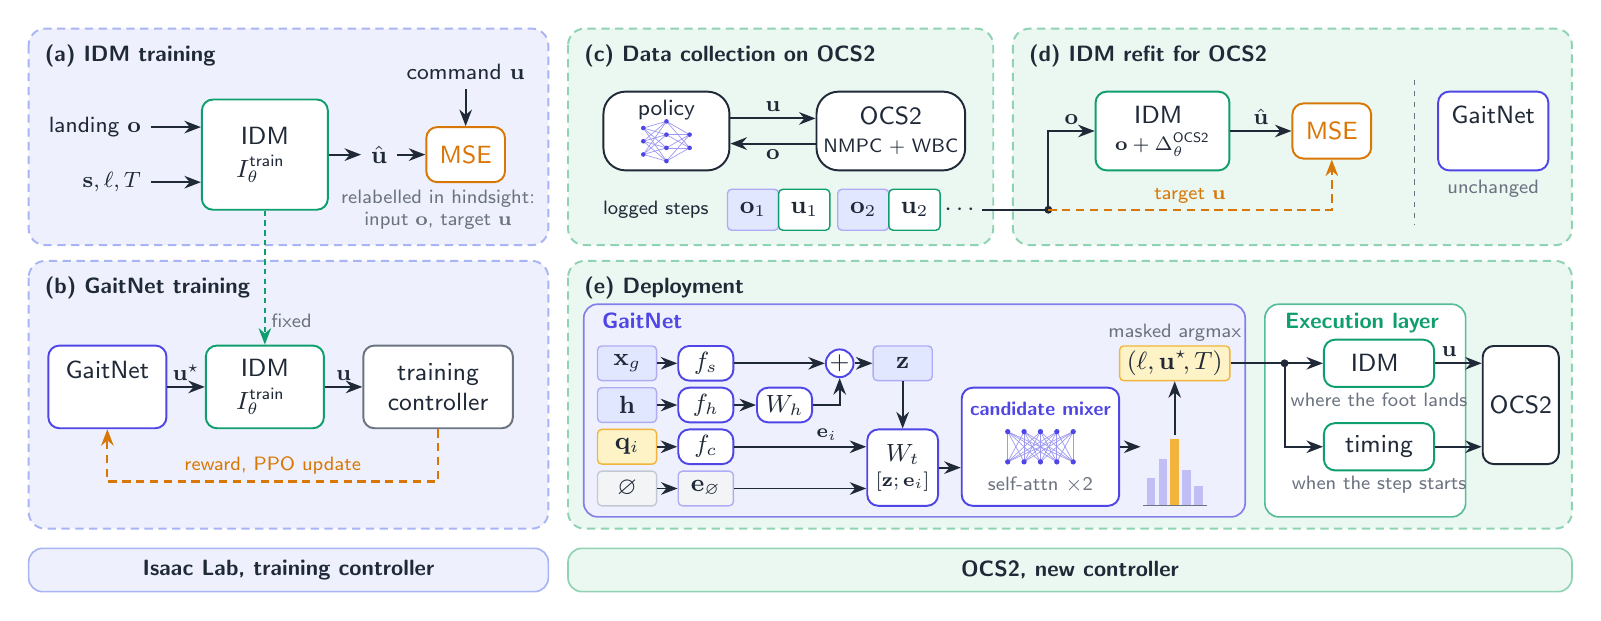
\begin{tikzpicture}[gfig]
% ---------------------------------------------------------------- panels
\draw[region={rgS}{rgSd}] (0,0)        rectangle (6.6,-2.75);    % (a)
\draw[region={rgS}{rgSd}] (0,-2.95)    rectangle (6.6,-6.35);    % (b)
\draw[region={rgG}{rgGd}] (6.85,0)     rectangle (12.25,-2.75);  % (c)
\draw[region={rgG}{rgGd}] (12.5,0)     rectangle (19.6,-2.75);   % (d)
\draw[region={rgG}{rgGd}] (6.85,-2.95) rectangle (19.6,-6.35);   % (e)
\node[ptitle] at (0.2,-0.2)   {(a) IDM training};
\node[ptitle] at (0.2,-3.15)  {(b) GaitNet training};
\node[ptitle] at (7.05,-0.2)  {(c) Data collection on OCS2};
\node[ptitle] at (12.7,-0.2)  {(d) IDM refit for OCS2};
\node[ptitle] at (7.05,-3.15) {(e) Deployment};
% domain bands
\draw[band={rgS}{rgSd}] (0,-6.6)    rectangle (6.6,-7.15);
\draw[band={rgG}{rgGd}] (6.85,-6.6) rectangle (19.6,-7.15);
\node[font=\sffamily\footnotesize\bfseries, text=ink] at (3.3,-6.875)
  {Isaac Lab, training controller};
\node[font=\sffamily\footnotesize\bfseries, text=ink] at (13.225,-6.875)
  {OCS2, new controller};

% ---------------------------------------------------------------- (a)
% IDM fitted by hindsight relabelling: input the landing o, target the
% command u that produced it.
\def\ya{-1.6}
\node[mod=acC, minimum width=16mm, minimum height=14mm] (ia) at (3.0,\ya)
  {IDM\\[1pt]$I^{\text{train}}_\theta$ \hot};
\node[font=\sffamily\footnotesize, anchor=east] (ao) at (1.55,{\ya+0.35}) {landing $\mathbf o$};
\node[font=\sffamily\footnotesize, anchor=east] (as) at (1.55,{\ya-0.35}) {$\mathbf s,\ell,T$};
\draw[arr] (ao.east) -- (ao.east -| ia.west);
\draw[arr] (as.east) -- (as.east -| ia.west);
\node (ua) at (4.45,\ya) {$\hat{\mathbf u}$};
\draw[arr] (ia) -- (ua);
\node[mod=acT, minimum width=10mm, text=acT] (ma) at (5.55,\ya) {MSE};
\draw[arr] (ua) -- (ma);
\node[font=\sffamily\footnotesize] (ta) at (5.55,-0.55) {command $\mathbf u$};
\draw[arr] (ta) -- (ma);
\node[sub] at (5.2,-2.3) {relabelled in hindsight:\\input $\mathbf o$, target $\mathbf u$};

% ---------------------------------------------------------------- (b)
% PPO with the training controller's IDM fixed between GaitNet and the
% (randomized) training controller.
\def\yb{-4.55}
\node[mod=acB, minimum width=15mm, minimum height=10.5mm] (gb) at (1.0,\yb) {GaitNet\\[1pt]\hot};
\node[mod=acC, minimum width=15mm, minimum height=10.5mm] (ib) at (3.0,\yb) {IDM\\[1pt]$I^{\text{train}}_\theta$ \frz};
\node[mod=muted, minimum width=19mm, minimum height=10.5mm] (cb) at (5.2,\yb) {training\\controller};
\draw[arr] (gb) -- node[above, alab] {$\mathbf u^\star$} (ib);
\draw[arr] (ib) -- node[above, alab] {$\mathbf u$} (cb);
\draw[tarr] (cb.south) -- (5.2,-5.75) -- node[above, tlab, text=acT]
  {reward, PPO update} (1.0,-5.75) -- (gb.south);
\draw[->, line width=0.7pt, draw=acC, dash pattern=on 2pt off 1.5pt]
  (ia.south) -- node[right, tlab, text=muted, pos=0.82] {fixed} (ib.north);

% ---------------------------------------------------------------- (c)
% A policy walks on OCS2 and every executed step is logged as (o, u).
\def\yc{-1.3}
\node[mod=ink, minimum width=16mm, minimum height=10mm, rounded corners=8pt] (pc) at (8.1,\yc) {};
\node[font=\sffamily\footnotesize] at (8.1,{\yc+0.27}) {policy};
\pic[scale=0.7] at (8.1,{\yc-0.13}) {mlp=acB};
\node[mod=ink, minimum width=17mm, minimum height=10mm, rounded corners=8pt] (oc) at (10.95,\yc)
  {OCS2\\[-1pt]{\scriptsize NMPC + WBC}};
\draw[arr] ([yshift=1.6mm]pc.east) -- node[above, alab] {$\mathbf u$} ([yshift=1.6mm]oc.west);
\draw[arr] ([yshift=-1.6mm]oc.west) -- node[below, alab] {$\mathbf o$} ([yshift=-1.6mm]pc.east);
\node[font=\sffamily\scriptsize, text=ink, anchor=west, inner sep=0pt] at (pc.west |- 0,-2.3) {logged steps};
\node[tok={tkS}{acB!45}, minimum width=6.5mm] at (9.2,-2.3)  {$\mathbf o_1$};
\node[tok={white}{acC},  minimum width=6.5mm] at (9.85,-2.3) {$\mathbf u_1$};
\node[tok={tkS}{acB!45}, minimum width=6.5mm] at (10.6,-2.3) {$\mathbf o_2$};
\node[tok={white}{acC},  minimum width=6.5mm] at (11.25,-2.3) {$\mathbf u_2$};
\node[inner sep=1pt] (dots) at (11.85,-2.3) {$\cdots$};

% ---------------------------------------------------------------- (d)
% The logged landing o is the IDM's input and the logged command u its
% target (hindsight relabelling, as in (a)); GaitNet is not retrained.
\def\yd{-1.3}
\node[mod=acC, minimum width=17mm, minimum height=10mm] (id) at (14.4,\yd)
  {IDM \hot\\[-1pt]{\scriptsize $\mathbf o + \Delta^{\text{OCS2}}_\theta$}};
\node[mod=acT, minimum width=10mm, text=acT] (md) at (16.55,\yd) {MSE};
\draw[arr] (id) -- node[above, alab] {$\hat{\mathbf u}$} (md);
\coordinate (jd) at (12.95,-2.3);
\draw[line width=0.7pt, draw=ink] (dots.east) -- (jd);
\fill[ink] (jd) circle (0.05);
\draw[arr] (jd) |- node[pos=0.75, above, alab] {$\mathbf o$} (id.west);
\draw[tarr] (jd) -| node[pos=0.25, above, tlab, text=acT] {target $\mathbf u$} (md.south);
\draw[muted, line width=0.6pt, dash pattern=on 2pt off 2pt] (17.6,-0.65) -- (17.6,-2.5);
\node[mod=acB, minimum width=14mm, minimum height=10mm] (gd) at (18.6,\yd) {GaitNet\\[1pt]\frz};
\node[sub, anchor=north] at (18.6,-1.88) {unchanged};

% ---------------------------------------------------------------- (e)
% GaitNet (frozen) as in Sec. III-B: context z = f_s(x_g) + W_h f_h(h);
% tokens W_t[z; e_i] with e_i = f_c(q_i) and a learned e_0 for no-step;
% candidate mixer; heads (alpha_i, T_i); masked argmax. The execution
% layer (Sec. III-C, III-E) sets where (IDM) and when (timing) the step
% is executed on OCS2.
\def\yA{-4.25} \def\yB{-4.78} \def\yC{-5.31} \def\yD{-5.84}
\def\yTop{-4.03} \def\yBot{-6.06}   % top of row A and bottom of row D tokens
\draw[fill=rgB, draw=acB!70, line width=0.6pt, rounded corners=5pt] (7.05,-3.5) rectangle (15.45,-6.2);
\node[font=\sffamily\footnotesize\bfseries, text=acB, anchor=north west, inner sep=0pt] at (7.275,-3.6) {GaitNet \frz};
% inputs
\node[tok={tkS}{acB!45}, minimum height=4.4mm] (xe) at (7.6,\yA) {$\mathbf x_g$};
\node[tok={tkS}{acB!45}, minimum height=4.4mm] (he) at (7.6,\yB) {$\mathbf h$};
\node[tok={tkC}{tkCd},   minimum height=4.4mm] (qe) at (7.6,\yC) {$\mathbf q_i$};
\node[tok={tkN}{rgAd},   minimum height=4.4mm] (ne) at (7.6,\yD) {$\varnothing$};
% context z = f_s(x_g) + W_h f_h(h)
\node[mod=acB, minimum width=7mm, minimum height=4.4mm, inner sep=1pt] (fse) at (8.6,\yA) {$f_s$};
\node[mod=acB, minimum width=7mm, minimum height=4.4mm, inner sep=1pt] (fhe) at (8.6,\yB) {$f_h$};
\node[mod=acB, minimum width=7mm, minimum height=4.4mm, inner sep=1pt] (whe) at (9.6,\yB) {$W_h$};
\node[draw=acB, circle, line width=0.7pt, fill=white, inner sep=0.2pt] (pe) at (10.3,\yA) {$+$};
\node[tok={tkS}{acB!45}, minimum height=4.4mm] (ze) at (11.1,\yA) {$\mathbf z$};
\draw[arr] (xe) -- (fse);  \draw[arr] (he) -- (fhe);
\draw[arr] (fse) -- (pe);  \draw[arr] (fhe) -- (whe);
\draw[arr] (whe.east) -| (pe.south);
\draw[arr] (pe) -- (ze);
% candidate embeddings and tokens [z; e_i]; W_t spans rows C-D
\node[mod=acB, minimum width=7mm, minimum height=4.4mm, inner sep=1pt] (fce) at (8.6,\yC) {$f_c$};
\node[tok={tkN}{acB!45}, minimum width=7mm, minimum height=4.4mm] (e0e) at (8.6,\yD) {$\mathbf e_\varnothing$};
\draw[arr] (qe) -- (fce);  \draw[arr] (ne) -- (e0e);
\node[mod=acB, minimum width=9mm, minimum height=9.7mm, inner sep=1pt] (wte) at (11.1,{(\yC+\yD)/2})
  {$W_t$\\[-2pt]{\scriptsize $[\mathbf z;\mathbf e_i]$}};
\draw[arr] (fce) -- node[above, alab, font=\scriptsize, pos=0.7] {$\mathbf e_i$} (fce -| wte.west);
\draw[arr] (e0e) -- (e0e -| wte.west);
\draw[arr] (ze) -- (wte);
% candidate mixer spans rows B-D
\node[mod=acB, minimum width=20mm, minimum height=15mm] (mxe) at (12.85,{(\yB+\yD)/2}) {};
\node[font=\sffamily\scriptsize\bfseries, text=acB] at (12.85,{\yB-0.05}) {candidate mixer};
\pic[scale=0.8] at (12.85,\yC) {attn=acB};
\node[sub] at (12.85,{\yD+0.05}) {self-attn $\times$2};
\draw[arr] (wte) -- (wte -| mxe.west);
% heads (alpha_i, T_i) on the row-D baseline, masked argmax up to row A
\begin{scope}[shift={(14.2,\yBot)}]
  \foreach \x/\hgt/\c in {0/0.35/acB!35, 0.15/0.6/acB!35, 0.3/0.85/tkCd, 0.45/0.45/acB!35, 0.6/0.25/acB!35}
    \fill[\c] (\x,0) rectangle ++(0.11,\hgt);
  \draw[muted, line width=0.4pt] (-0.05,0) -- (0.76,0);
\end{scope}
\draw[arr] (mxe.east |- 0,\yC) -- (14.12,\yC);
\node[tok={tkC}{tkCd}, minimum width=14mm, minimum height=4.4mm] (se) at (14.555,\yA) {$(\ell,\mathbf u^\star\!,T)$};
\node[sub, anchor=south] at (14.555,{\yTop+0.02}) {masked argmax};
\draw[arr] (14.555,{\yBot+0.9}) -- (se);
% execution layer: where (IDM, row A) and when (timing, row C)
\draw[fill=white, draw=acC!70, line width=0.6pt, rounded corners=5pt] (15.7,-3.5) rectangle (18.25,-6.2);
\node[font=\sffamily\footnotesize\bfseries, text=acC, anchor=north west, inner sep=0pt] at (15.95,-3.6) {Execution layer};
\coordinate (je) at (15.95,\yA);
\draw[line width=0.7pt, draw=ink] (se.east) -- (je);
\fill[ink] (je) circle (0.05);
\node[mod=acC, minimum width=14mm, minimum height=6mm] (ie) at (17.15,\yA) {IDM \frz};
\node[sub, anchor=north] at (17.15,{\yA-0.33}) {where the foot lands};
\node[mod=acC, minimum width=14mm, minimum height=6mm] (tie) at (17.15,\yC) {timing};
\node[sub, anchor=north] at (17.15,{\yC-0.33}) {when the step starts};
\draw[arr] (je) -- (ie);
\draw[arr] (je) |- (tie.west);
% OCS2 receives the command and the start time; centred on row B
\node[mod=ink, minimum width=9.5mm, minimum height=15mm] (oe) at (18.95,\yB) {OCS2};
\draw[arr] (ie.east) -- node[pos=0.3, above, alab] {$\mathbf u$} (ie.east -| oe.west);
\draw[arr] (tie.east) -- (tie.east -| oe.west);
\end{tikzpicture}%
}
\caption{GaitNet pipeline. (a)~An inverse footstep model (IDM) for the
  training controller is fitted on its logged steps: given where a foot
  landed, it predicts the command that put it there. (b)~GaitNet is
  trained with PPO, with this IDM fixed between GaitNet and the
  controller. (c)~On a new controller, OCS2, steps are logged
  again\pending{ (policy to be added)}, and (d)~a new IDM is fitted on
  them while GaitNet stays frozen. (e)~At deployment, GaitNet encodes the
  state $\mathbf x_g$ and its recent motion $\mathbf h$ into a context
  $\mathbf z$, scores each safe candidate $\mathbf q_i$ and the no-step
  option $\varnothing$ in a candidate mixer, and picks one step
  $(\ell,\mathbf u^\star\!,T)$ (Fig.~\ref{fig:architecture}). The
  execution layer then sets where and when OCS2 executes it: the OCS2 IDM
  turns $\mathbf u^\star$ into a command $\mathbf u$, and the step is
  written into OCS2's schedule a fixed lead after the decision.
  \hot~trained; \frz~frozen.}
\label{fig:overview}
\end{figure*}


Legged robots can cross broken or narrow terrain that stops wheels
and tracks, as long as they find where to place their feet.
Choosing those footholds is only part of the problem: the robot must
also decide which legs to move, when to lift them, and how long its swings
should last. Together, these decisions are called
\emph{contact planning}. Most controllers simplify contact planning
with a fixed gait, which sets the leg timing and ordering in advance but cannot
react when safe footholds appear at irregular places and times.
Learned footstep planners can make these choices implicitly, and
simulation lets them practice on large amounts of terrain. Yet a learned planner is trained on top of one low-level controller and
then deployed on another, and a controller does not always place the
foot where it is told. Our \emph{training controller}, for example,
lands the foot a few centimeters off of the commanded target, which is more than the safety margin around terrain elements.
\emph{OCS2} \cite{ocs2}, a nonlinear model predictive controller
(NMPC) with whole-body control (WBC), misses in a different way and
also starts each step on its own schedule. When a learned planner fails
on a new controller, the fault therefore need not lie in choosing a
safe foothold; it can lie in landing on it.

Model-based planners place
foothold choice, contact timing, and whole-body motion inside one
model predictive controller \cite{Wensing2022Nov}. This works well
when the contact pattern is known, but once the planner must choose
contacts, the problem becomes a mixed-integer program. Some methods
reduce the search by limiting footholds to convex terrain regions
\cite{deits_footstep_2014}, and others optimize contact schedules and
timing together \cite{winkler_gait_2018}. Gait-free planners remove the
periodic schedule altogether, choosing contact timing online from
% placeholder image
\begin{figure}[H]
    \centering
    \includegraphics[width=0.5\textwidth]{example-image-a}
    \caption{Robot navigating challenging terrain.}
    \label{fig:placeholder}
\end{figure}
per-leg feasibility rules \cite{bjelonic_whole-body_2021} or by tree
search \cite{amatucci_monte_2022}, and recent work speeds up this
search by learning its cost-to-go \cite{taouil_non-gaited_2024} or by
learning per-foot flight phases inside an MPC horizon
\cite{patrizi_rl-augmented_2026}. These planners decide contact
timing, but not footholds chosen from a perceived map of safe cells.

Learned planners make the contact decision instead. End-to-end
policies put it inside one neural controller and cross hard terrain
reliably \cite{lee_learning_2020, zhang_learning_2023}; trained
without an explicit schedule, they can even develop gaits on their own
\cite{fu_minimizing_2021}. Their contact decision, however, is hidden
inside the joint targets, so it cannot be checked before execution or
handed to a model-based controller. Perceptive model-based stacks
instead project an explicit foothold onto a convex terrain region
\cite{grandia_perceptive_2022}, and hybrid methods learn that foothold
while a gait generator still fixes the timing
\cite{gangapurwala_rloc_2022, tsounis_deepgait_2020}. The closest
work, ContactNet \cite{bratta_contactnet_2024}, ranks discretized
foothold candidates with a network without prescribing which leg
swings. Its concurrency, however, is set by configuration, it re-ranks
candidates only at touchdown, and its gait sets the swing timing.

Finally, work on moving learned policies to new robots or domains has
moved body motion, joint actions, or footholds within a fixed gait,
but not gait-free footstep choices. Li et al.
\cite{li_zero-shot_2022} retarget learned quadruped locomotion
policies to new robots through a hybrid kinodynamic MPC, and RLOC
\cite{gangapurwala_rloc_2022} moves its learned footstep policy to a
larger robot while keeping its gait. Xie et al. \cite{xie_fada_2026}
split a humanoid policy into a planner, which states the intended
motion, and an inverse dynamics model, which turns it into actions,
and then adapt only the inverse model to a new domain.

We present GaitNet (Fig.~\ref{fig:overview}), which separates choosing
a step from executing it. Every \emph{tick}, the planner picks one step
or a \emph{no-step option} from a few safe \emph{candidate} footholds
per leg, kept away from \emph{voids}, the holes in the ground. Because
a controller may not place the foot where it is told, an execution
layer then makes the controller land each step where and when the
planner meant. On the training controller, this layer is an
\emph{inverse footstep model} (IDM), fitted from the controller's own
logged steps, which turns where GaitNet wants the foot into the command
that lands it there. For a new controller, the IDM is refit on that
controller's own logged steps, and on OCS2 steps are also delivered on
OCS2's own schedule. GaitNet is trained in Isaac Lab
\cite{mittal_orbit_2023} and is never retrained. It builds on the
one-step-per-tick action space of \cite{Sullivan2025}, which was tested
on one controller; the candidate attention, the motion history, the
execution layer, the second controller, and all results are new here,
and all results are in simulation.

% Kept in one block so the list never breaks across columns or pages.
% NOTE (owen): we'll want to re-condiser this later. as of now, it left a huge gap on pg2
% \noindent\begin{minipage}{\linewidth}
Our contributions are:
\begin{itemize}
  \item GaitNet, a footstep planner that is given no gait. Every tick, it
    picks one step or none from sampled safe footholds, comparing the
    candidates with attention and using a short motion history
    (Secs.~\ref{subsec:method-step} and~\ref{subsec:method-network}).
  \item An execution layer that lets the frozen GaitNet run on a new
    controller, with an inverse footstep model per controller fitted by
    hindsight relabelling from that controller's own logged steps
    (Secs.~\ref{subsec:method-idm} and~\ref{subsec:method-deployment}).
  \item An evaluation on OCS2 with a simulated depth camera, over
    0--\corlOcsMaxVoidPct\% voids and
    \corlOcsSpeedMin--\corlOcsSpeedMax\,m/s, in which GaitNet matches
    OCS2's own trot on sparse voids and exceeds it on dense voids and
    at faster commands, and ablations of overlapping swings, the IDM,
    and the candidate comparison (Sec.~\ref{sec:experiments}).
\end{itemize}
% \end{minipage}

\section{Problem Setup}
\label{sec:setup}

We study footstep planning for a Unitree Go1 quadruped walking forward
over ground with voids. At a fixed rate, a planner decides whether to
start a step and which one, and a low-level controller executes it.

At each tick, the planner observes the
robot's state, a set
$\mathcal C$ of candidate footholds, and a short history of the
robot's motion. It returns either the no-step option or a step
$(\ell, \mathbf u^\star, T)$: a leg $\ell$, a landing point
$\mathbf u^\star \in \mathcal C$, and a swing time $T$. The landing
point is an offset from the leg's hip in the yaw frame, the
gravity-aligned frame that turns with the robot's heading, taken at
the moment of the decision.

To execute the step, a controller $c$ receives a command $\mathbf u$,
also an offset from the hip in this yaw frame, and a start time. Sent
$\mathbf u$ for leg $\ell$ and swing time $T$ in robot state
$\mathbf s$, it lands the foot at
\begin{equation}
  \mathbf o = F_c(\mathbf s, \ell, T, \mathbf u)
    = \mathbf u + \boldsymbol\delta_c(\mathbf s, \ell, T, \mathbf u),
  \label{eq:forward}
\end{equation}
where $\boldsymbol\delta_c$ is the controller's landing error. Both
$\boldsymbol\delta_c$ and the controller's step timing differ between
controllers, and in general $\boldsymbol\delta_c \neq \mathbf 0$
(Sec.~\ref{subsec:method-idm}). An execution layer therefore sits
between the planner and the controller and turns each step into a
command and a start time for controller $c$.

We train the planner in
Isaac Lab with the \emph{training controller}, the convex MPC of Di
Carlo et al.\ \cite{dicarlo_dynamic_2018}, to follow a
forward velocity command over terrain with voids without falling
(Sec.~\ref{subsec:method-training}). We then freeze the planner's
weights and run it with OCS2
(Sec.~\ref{subsec:method-deployment}). Only the execution layer is
refit for the new controller. The goal is success on held-out
worlds comparable to that of OCS2's own gait.

\section{GaitNet}
\label{sec:method}

GaitNet has two parts (Fig.~\ref{fig:overview}). A planner chooses, at
every tick, which step to take, if any, and an execution layer turns
that step into a command that the controller in use lands where and
when the planner meant. Table~\ref{tab:settings} lists the main
settings.

\subsection{Choosing One Step per Tick}
\label{subsec:method-step}

GaitNet chooses steps one at a time, and often enough to change its
plan while a leg is still in the air. At every tick it may start at
most one step for one leg, while the other legs keep their current
commands. A swing lasts several ticks, so GaitNet may start a second
swing before the first one ends. Two feasibility rules decide which
legs may step: a leg that is already swinging cannot be chosen, and a
new step needs at least \numberstringnum{\corlMinContactLegs} legs in
scheduled stance, where a leg that is waiting to lift off counts as
lifted. At most \numberstringnum{\corlMaxConcurrentSwingLegs} legs
therefore swing at once. Beyond these rules, GaitNet never chooses a
gait phase, leg pair, or contact sequence. It is \emph{greedy},
committing only to the next step, and the contact sequences it
produces are \emph{acyclic}, following neither a gait cycle nor a gait
library; the literature also calls them \emph{non-gaited} or
\emph{free-gait}. At each tick, it simply asks whether any available
step is better than doing nothing. If one is and another leg is
already in the air, the swings overlap; if the no-step option wins,
the robot waits.

The candidates are safe cells near each hip. A grid of terrain rays around the hip marks a cell as safe
when the ground under it is within reach below the hip, and as unsafe
when it is a void or the ray misses. The unsafe cells are then grown
by \numberstringnum{\corlMarginCm} cells, so that no remaining safe
cell lies within \corlMarginCm\,cm of a void; no other reach, edge, or
kinematic rule is applied. For each leg that may step, GaitNet draws a
fixed number of safe cells at random, without repeats, and masks the
empty slots when a leg has fewer. Together with the no-step option,
these candidates form the \emph{choices} of a tick, the same set in
training and at deployment.

\subsection{GaitNet Architecture}
\label{subsec:method-network}

GaitNet turns the robot state, the candidate set, and the recent motion
into one score and one swing time per choice (Fig.~\ref{fig:overview}a).

GaitNet has three inputs. The first is the tracking state
\begin{equation}
  \mathbf{x_g} =
  \begin{bmatrix}
    \mathbf p_{f,xy}^{b} &
    p_{b,z} &
    \mathbf v_b &
    \boldsymbol\omega_b &
    \mathbf v^{usr} &
    \mathbf c &
    \mathbf g_b
  \end{bmatrix}^T ,
  \label{eq:gaitnet-x}
\end{equation}
which holds the $xy$ positions of the four feet relative to the trunk
($\mathbf p_{f,xy}^{b}$), the base height in the world frame
($p_{b,z}$), the base linear and angular velocity ($\mathbf v_b$,
$\boldsymbol\omega_b$), the velocity command ($\mathbf v^{usr}$), the
controller's \emph{scheduled} contact rather than a sensed one
($\mathbf c$), and projected gravity ($\mathbf g_b$); all vectors
except $p_{b,z}$ are in the trunk frame. The second input is the
set of $N$ candidates and the no-step option $\varnothing$. Candidate
$i$ is described by a vector $\mathbf q_i$: a one-hot code for its leg
and its offset from the hip; the no-step option has its own code. A last entry, a cost from a separate network in
\cite{Sullivan2025}, is kept at zero, because zeroing it improved
survival there. The third input is the
history $\mathbf h$ of the last second of motion. Each of its ticks
holds the base velocities, each foot's position relative to its hip
from the joint encoders, the scheduled contact, and each leg's last
\emph{touchdown error}, which is where the foot was at its scheduled
touchdown minus the command. All inputs are available on a real robot.

GaitNet first combines these inputs. A state encoder $f_s$ and a
history encoder $f_h$ build a context vector
\begin{equation}
  \mathbf z = f_s(\mathbf x_g) + W_h\, f_h(\mathbf h),
  \label{eq:context}
\end{equation}
where $W_h$ is a linear projection. A candidate encoder $f_c$, shared by
all candidates, embeds each candidate as $\mathbf e_i = f_c(\mathbf q_i)$,
and the no-step option has a learned embedding $\mathbf e_\varnothing$
instead. Each choice then becomes a token
$\mathbf t_i = \mathrm{ReLU}(W_t [\mathbf z; \mathbf e_i])$ that
combines the shared context with that choice.

So that a choice can be judged
against the alternatives, a \emph{candidate mixer} $M$ lets the tokens
attend to each other. It is a small pre-norm transformer encoder
\cite{vaswani_attention_2017}: each layer updates every token as
$\mathbf t \leftarrow \mathbf t + \mathrm{MHA}(\mathrm{LN}(\mathbf t))$
and then $\mathbf t \leftarrow \mathbf t + \mathrm{FF}(\mathrm{LN}(\mathbf
t))$, with multi-head attention MHA, layer normalization LN, and a
feed-forward block FF. Empty slots are masked as keys, so no token
attends to them, while the no-step option is visible to all.

After the mixer, a readout $g$ maps each mixed token
$\tilde{\mathbf t}_i$ to a feature $\mathbf y_i = g(\tilde{\mathbf t}_i)$,
from which two linear heads give a score and a swing time,
\begin{equation}
  \alpha_i = \mathbf w_\alpha^\top \mathbf y_i, \qquad
  T_i = T_{\min} + (T_{\max} - T_{\min})\,
    \sigma(\mathbf w_T^\top \mathbf y_i),
  \label{eq:heads}
\end{equation}
where $\sigma$ is the logistic function and $[T_{\min}, T_{\max}]$ is
the allowed swing-time range.

The scores of the valid choices are the
logits of a categorical distribution $\pi(i) \propto \exp(\alpha_i)$;
empty slots get zero probability, and the no-step option is always
allowed. In training, GaitNet samples a choice $i$ and then a swing
time $T \sim \mathcal N(T_i, \sigma_T^2)$ with a small fixed
$\sigma_T$, and the log probability of the action is
$\log \pi(i) + \log \mathcal N(T; T_i, \sigma_T^2)$. At deployment it
takes the top-scoring choice and its mean swing time $T_i$, and issues
no step if the no-step option wins.

GaitNet starts training as a simpler network. The projection $W_h$, the attention output projections, and the last layer
of each feed-forward block start at zero. At initialization, the mixer
is therefore the identity and the context ignores the history, so every
choice is scored on its own from $\mathbf x_g$ and $\mathbf q_i$.
GaitNet then computes exactly the \emph{per-candidate network} of
\cite{Sullivan2025}, whose trunk corresponds to our token layer and readout. During training, GaitNet
learns to use the history and to compare candidates; afterwards, a
candidate's score depends on the whole candidate set, so GaitNet runs
on the same sampled set at deployment as in training.

\subsection{Inverse Footstep Model}
\label{subsec:method-idm}

The execution layer is needed because a controller does not always
place the foot where it is told, and each controller misses in its own
way. Our training controller keeps re-aiming each swing at the moving
hip, so the foot lands past the commanded point, and the faster the
robot walks, the farther past it lands. Without correction, we measure
a shift of +\corlOvershootSlowMin{} to +\corlOvershootSlowMax\,cm along
the walking direction at \corlSimSpeedSlow\,m/s and
+\corlOvershootFastMin{} to +\corlOvershootFastMax\,cm at
\corlSimSpeedFast\,m/s, against the \corlMarginCm\,cm margin that
GaitNet keeps around voids. OCS2, in contrast, fixes the target in the
world when the step is commanded.

We therefore fit one inverse footstep model (IDM) per controller. For
controller $c$, the IDM $I^c$ approximates the inverse of $F_c$ in
Eq.~\eqref{eq:forward}, $\mathbf u \approx I^c(\mathbf s, \ell, T,
\mathbf o)$. GaitNet's chosen candidate $\mathbf u^\star$ is a cell it
judged safe to land on, so we treat it as the desired landing and send
\begin{equation}
  \mathbf u = I^c(\mathbf s, \ell, T, \mathbf u^\star),
  \qquad\text{so that}\qquad
  F_c(\mathbf s, \ell, T, \mathbf u) \approx \mathbf u^\star .
  \label{eq:idm}
\end{equation}
GaitNet is the same for every controller; only $I^c$ changes. This
split into a planner and an inverse model follows Xie et al.\
\cite{xie_fada_2026}.

The IDM itself is a small network that predicts a correction to the desired
landing,
\begin{equation}
  I^c_\theta(\mathbf s, \ell, T, \mathbf o) =
  \mathbf o + \Delta^c_\theta(\mathbf h_{\text{last}}, \ell, T, \mathbf o),
  \label{eq:idm-model}
\end{equation}
where $\mathbf h_{\text{last}}$, the newest tick of GaitNet's history,
stands in for the robot state, and $\Delta^c_\theta$ is a small MLP.
The last layer of $\Delta^c_\theta$ starts at zero, so an untrained IDM
is the identity and sends GaitNet's choice unchanged.

We fit each IDM by hindsight relabelling. We log steps that its
controller actually executes, each as a tuple
$(\mathbf s, \ell, T, \mathbf u, \mathbf o)$. Whatever the command
$\mathbf u$ was aimed at, it is by definition a command that lands the
foot at $\mathbf o$, so the pair from $\mathbf o$ to $\mathbf u$ is a
correct example of the inverse map. We therefore fit
\begin{equation}
  \min_\theta \; \mathbb E\,
  \big\| \mathbf u - I^c_\theta(\mathbf s, \ell, T, \mathbf o) \big\|^2
  \label{eq:idm-loss}
\end{equation}
by supervised regression. For the training controller, the steps come
from two earlier policies without randomization, at up to 30\% voids
and across our speed range; a policy's own commands cover only the
footholds it prefers, so we add Gaussian noise to every command to
widen the data around them. For OCS2, we log the steps of the frozen
GaitNet, run on OCS2 with the training controller's IDM, on world seeds
61--110, fewer than 20{,}000 steps in all.

\subsection{Training GaitNet with the IDM}
\label{subsec:method-training}

We train GaitNet, as the actor, with Proximal Policy Optimization (PPO)
\cite{Schulman_proximal_2017} in Isaac Lab \cite{mittal_orbit_2023},
with many robots in parallel and the training controller's IDM, fixed,
between GaitNet and the controller. The critic is
a separate, smaller network that reads the state and the candidates,
but not the history, and shares no weights with the actor; it scores
each choice, and a small MLP maps these scores to one state value.

\begin{table}[t]
  \centering
  \caption{Main settings}
  \label{tab:settings}
  \footnotesize
  \setlength{\tabcolsep}{3pt}
  % source: gaitnet-docs/methodology.md 3-6, training-setup.md 5-10,
  % experiment-setup.md 2. Full settings: gaitnet-docs (supplementary).
  \begin{tabular*}{\columnwidth}{@{\extracolsep{\fill}}ll@{}}
    \toprule
    \thd{Item} & \thd{Value} \\
    \midrule
    \grouprow{2}{GaitNet}
    Tick; swing time & \corlControlTickMs\,ms;
      \corlSwingDurationMin--\corlSwingDurationMax\,s \\
    Candidates per leg; choices & \corlTrainCandidatesPerLeg;
      \corlTotalCandidates{} with no-step \\
    Candidate grid; void margin & $\pm\corlGridReachCm$\,cm at
      \corlScanResCm\,cm; \corlMarginCm\,cm \\
    History & \corlHistSeconds\,s (\corlHistTicks{} ticks) \\
    Candidate mixer & \corlMixerLayers{} layers, width \corlMixerDim,
      \corlMixerHeads{} heads \\
    Parameters & \corlParamsGaitNetK{}k (per-candidate:
      \corlParamsPerCandidateK{}k) \\
    \grouprow{2}{Inverse footstep model}
    Network; data & MLP, 2 $\times$ \corlIdmHidden;
      \corlIdmFootsteps{} steps \\
    Held-out error & \corlIdmRmsCm\,cm RMS (\corlIdmIdentityRmsCm\,cm
      uncorrected) \\
    \grouprow{2}{Training (Eq.~\eqref{eq:reward})}
    Robots; rollout; learning rate & \corlParallelEnvs;
      \corlRolloutSteps{} steps; $\corlLearningRate$ \\
    $w_a$; $w_s$; $w_f$ & \corlAliveWeight; \corlActionPenalty;
      \corlTerminationPenalty \\
    $\sigma_v$; $\sigma_\omega$; $\sigma_T$ & \corlTrackXyStd\,m/s;
      \corlTrackYawStd\,rad/s; \corlDurationExploreStd\,s \\
    Curriculum & \corlNumLevels{} levels, 0--\corlMaxVoidPct\% voids \\
    \grouprow{2}{OCS2}
    Step lead & \corlGzLead\,s \\
    \bottomrule
  \end{tabular*}
\end{table}


The training task is to walk over ground with voids. The terrain is a grid of cells, a
fraction of which, the \emph{void fraction}, are deep voids. The robot
must follow a forward velocity command until a time-out; it fails
earlier if the trunk tilts or drops too far, or if a foot drops below
the ground, which means a foot in a void. Commands are forward-only
because the deployed robot maps terrain with a forward-facing camera.
The reward per tick is
\begin{multline}
  r = \Delta t\,\Big[\,w_a\,\mathbb{I}_{\text{alive}}
  + e^{-\|\mathbf v^{usr}_{xy} - \mathbf v_{b,xy}\|^2/\sigma_v^2}
  + e^{-(\omega^{usr}_z - \omega_{b,z})^2/\sigma_\omega^2} \\
  - w_s\,\mathbb{I}_{\text{step}}
  - w_f\,\mathbb{I}_{\text{fail}}\Big],
  \label{eq:reward}
\end{multline}
where $\Delta t$ is the tick, superscript $usr$ marks the commanded
planar and yaw velocities, and subscript $b$ the matching base
velocities. There are no gait, clearance, posture, or smoothness
terms. The tracking widths $\sigma_v$ and $\sigma_\omega$ are narrow
on purpose: with Isaac Lab's default width, a robot standing still
would still earn most of the tracking reward at our speeds.
Observations are not normalized and carry no added noise, and there
are no pushes.

To make this task gradually harder, difficulty levels
raise the void fraction step by step. Isaac Lab's default curriculum
kept every robot on the lowest level at our speeds, so a robot instead
\emph{progresses} if it walks a set share of the commanded distance.
It moves up with probability $p_{\text{up}}$ after a progressing
time-out and down with probability $p_{\text{down}}$ after a failure
or a stalled time-out, so the share of failed or stalled episodes
settles near $p_{\text{up}}/(p_{\text{up}} + p_{\text{down}}) = 1/4$.
Each robot's controller is also redrawn at every reset, so GaitNet sees
a spread of tracking quality, swing heights, landing errors, and
lift-off delays.

The IDM is fitted first, offline (Sec.~\ref{subsec:method-idm}), and
then held fixed, so GaitNet and the IDM are not trained concurrently.
During GaitNet's training, every chosen candidate passes through the
training controller's IDM before the controller adds its randomized errors, although
the IDM itself was fitted without them. GaitNet still sees the raw
candidates, and its touchdown errors are measured against the IDM's
output, so its history reports how far the controller missed the
corrected command.

\subsection{Deployment on OCS2}
\label{subsec:method-deployment}

On OCS2, GaitNet replaces the gait scheduler of the
\texttt{legged\_control} stack \cite{leggedcontrol,
grandia_perceptive_2022} in Gazebo, where OCS2's NMPC \cite{ocs2}
plans the motion and a weighted WBC tracks it. A gait node asks a
GaitNet service for a decision every tick, also while two legs swing.
The service builds the same kind of candidate set, with a slightly
larger margin, rebuilds the history with the training code, and
applies the IDM fitted on OCS2's own steps (Sec.~\ref{subsec:method-idm}).

The IDM fixes where the foot lands; when a step starts is set by how
steps are delivered to OCS2, which also starts each step on its own
schedule. Each step is therefore written into OCS2's contact schedule
at absolute times on the NMPC clock, starting a fixed lead after the
decision, and is merged with the steps already planned. The body reference also stays a short distance ahead of the
body, and OCS2 runs with its stock task settings.

On OCS2, GaitNet and the controller get terrain either from
the world's exact geometry or from a simulated RealSense D435 depth
camera. For the camera, we build a \emph{depth-vote terrain}: a fine
grid in which each depth frame votes hit or miss for the cells it
sees. A cell is walkable while its fading votes are positive and it is
far enough from unwalkable cells, a distance that grows with how far
the robot has walked since it last saw the cell. The simulated depth images carry no noise. Odometry comes from OCS2's leg-based
state estimator with a \emph{slip gate}, which ignores feet whose
velocity disagrees with the estimate.

% Section IV: GaitNet on OCS2, from the benchmark the author sent on
% 2026-10-14 (OCS2-fitted IDM, depth-camera terrain, 0-70 % voids,
% 0.05-0.25 m/s, 10 trials per cell). Plots: figures/ocs2_results.pdf, made
% by figures/plot_ocs2_results.py, which holds the per-cell data. Pooled
% values: \corlOcs* macros in constants.tex.

\section{Simulation Experiments}
\label{sec:experiments}

We ask three questions. (Q1)~Does the frozen GaitNet succeed on OCS2 as
often as OCS2's own trot as voids get denser and commands faster?
(Q2)~Does GaitNet need to swing more than one leg at a time?
(Q3)~Do the IDM and the candidate mixer matter?

\subsection{Setup}
\label{subsec:exp-setup}

We deploy iteration \corlTrainingIterations{} of one training run, frozen
after training \verify{(to be confirmed for the OCS2 benchmark)}. The
run's settings changed while it trained. It used omnidirectional
commands for its first \corlOmniIterations{} iterations, then forward
commands without the IDM until iteration \corlIdmStartIteration, and
with the IDM in the loop after that. It was not seeded and used
$\corlTotalTransitions$ transitions, about \corlTrainHours\,h on one
NVIDIA RTX PRO 6000.

We run GaitNet on OCS2 in Gazebo (Sec.~\ref{subsec:method-deployment}),
with terrain from the simulated depth camera and the IDM fitted on
OCS2's own steps (Sec.~\ref{subsec:method-idm}). Each world is a strip
of pillars in which each tile is a real drop with probability equal to
the void fraction. We test eight void fractions, from 0 to
\corlOcsMaxVoidPct\%, and five forward speeds, from \corlOcsSpeedMin{}
to \corlOcsSpeedMax\,m/s, with \corlOcsTrialsPerCell{} trials for each
pair, and 14 for OCS2's own trot in the comparison by speed. The fastest command lies above the \corlCmdVxMax\,m/s that
GaitNet was trained on. A trial succeeds if the robot does not fall and
walks at least half the commanded distance \verify{(trial length to be
stated)}; leaving the strip also counts as a failure.
\pending{The benchmark's world seeds will be listed.}

We compare five conditions. All except OCS2's own trot keep OCS2's NMPC
and WBC but replace its gait scheduler and foothold choice with the
planner's steps, so the comparison focuses on the planner rather than
the tracker.
\begin{enumerate}
  \item GaitNet: as deployed; up to two legs may swing at once.
  \item OCS2's own trot: OCS2's perceptive trot, with its own gait
    scheduler and footholds \verify{(on the same camera)}.
  \item GaitNet-Single: only one leg may swing at a time.
  \item GaitNet, no IDM: the chosen landing point is sent to OCS2
    unchanged.
  \item Per-candidate + IDM: the per-candidate network of
    \cite{Sullivan2025} (Sec.~\ref{subsec:method-network}), which scores
    each candidate on its own, with the same IDM \verify{(checkpoint to
    be stated)}.
\end{enumerate}
\verify{GaitNet-Single and GaitNet, no IDM use GaitNet's weights.}

\begin{figure*}[t]
  \centering
  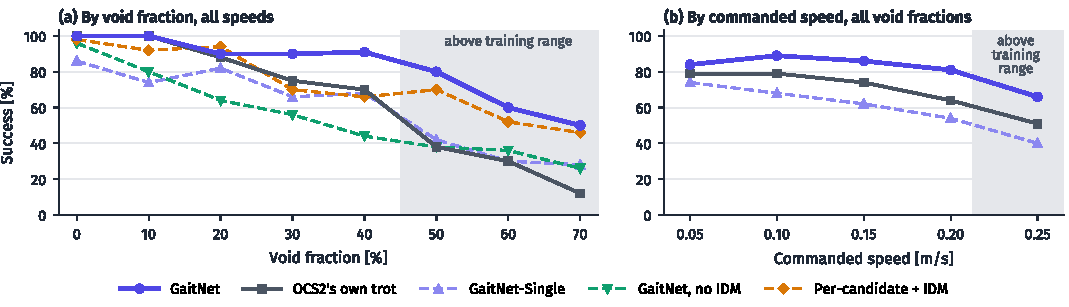
\includegraphics[width=\textwidth]{figures/ocs2_results}
  \caption{Success on OCS2 with depth-camera terrain. (a)~By void
    fraction, pooled over the five commanded speeds (50 trials per
    point). (b)~By commanded speed, pooled over the eight void fractions
    (80 trials per point, 112 for OCS2's own trot); GaitNet was trained up to
    \corlCmdVxMax\,m/s.}
  \label{fig:ocs2-results}
\end{figure*}

\subsection{Comparison with OCS2's Own Trot}
\label{subsec:exp-transfer}

GaitNet matches OCS2's own trot on sparse voids and does better as the
voids get denser (Fig.~\ref{fig:ocs2-results}a). Both succeed in every
trial up to 10\% voids and are within two points at 20\%. From 30\% voids on,
GaitNet leads at every void fraction, with \corlOcsDenseFull\% against
\corlOcsDenseTrot\% success over 40--\corlOcsMaxVoidPct\% voids.
At \corlOcsMaxVoidPct\% voids, GaitNet still succeeds in half of the trials and OCS2's own trot in few. GaitNet also leads at every
commanded speed (Fig.~\ref{fig:ocs2-results}b) and walks closer to
the commanded speed, at about 92\% of it against about 84\% for
OCS2's own trot \verify{(mean over trials)}. Both lose success at
\corlOcsSpeedMax\,m/s, above GaitNet's training range.

\subsection{Ablations}
\label{subsec:exp-why}

Overlapping swings matter (Q2). Under a one-swing limit, GaitNet still
walks, but it succeeds less often at every void fraction and every
speed, \corlOcsAllSingle\% against \corlOcsAllFull\% on average over
void fractions, and the gap is largest on dense voids and at the
faster commands. Because GaitNet was never trained under this limit,
this shows that GaitNet relies on occasionally swinging two legs
together, not that overlap is better in general.

The IDM matters most (Q3). Without it, GaitNet's success falls from
\corlOcsAllFull\% to \corlOcsAllNoIdm\% on average over void fractions.
Only on ground without voids, where a missed landing costs little,
does GaitNet do well without it.

Comparing candidates matters on dense voids. The per-candidate network,
which has neither the candidate mixer nor the history, with the same IDM, is about as good as GaitNet up to 20\% voids but
falls behind from 30\% on, with \corlOcsDenseMlp\% against
\corlOcsDenseFull\% over 40--\corlOcsMaxVoidPct\% voids. \verify{The two
networks also differ in training history}, so this is not a fully
controlled comparison.

\section{Conclusion}
\label{sec:conclusion}

We presented GaitNet, a footstep planner that is given no gait and
that separates choosing a step from executing it. GaitNet picks one
step per tick from sampled safe footholds, and an execution layer
makes each controller land that step where and when GaitNet meant.
Trained on one controller and run with its weights frozen on OCS2,
GaitNet succeeds about as often as OCS2's own trot on held-out worlds
with exact terrain, at the lower of our two speeds. In our pair of
controllers, the obstacles we found lay in execution rather than in
the choice of step: correcting only the landing point recovers an
earlier planner at speed on its own controller, and on OCS2 the
largest obstacle was when steps were delivered. Separating what to
step on from how a controller lands the foot there thus appears to be
a practical way to reuse a learned footstep planner across
controllers.

\section{Limitations}
\label{sec:limitations}

\pending{All results are in simulation; GaitNet has not yet run on a
Unitree Go1.} Within simulation, we moved GaitNet between only one pair
of controllers, and the OCS2 comparison uses \corlGzTrialsPerArm{}
trials per condition, which cannot separate GaitNet from OCS2's own
trot. The execution layer was also tuned with the same policy, and GaitNet
did worse than OCS2's own trot on flat ground at the faster speed
(Sec.~\ref{subsec:exp-transfer}). Nor have we ablated the execution layer on OCS2: we have
not run GaitNet there without anchoring, or with a simple hand-made
correction of the landing shift in place of the learned IDM, which
would show how much of the gain needs learning at all. At
\corlGzSpeed\,m/s the landing shift is also small, so our OCS2 tests
do not stress it. \pending{The OCS2 results reported here still use the training
controller's IDM.} Refitting the IDM requires logging steps on each new
controller first; adapting it online, in the spirit of
\cite{xie_fada_2026}, could remove that step.

The evidence for GaitNet's design is also incomplete. The value of the
candidate mixer and the history is not isolated: with the IDM, the
per-candidate network is within noise of GaitNet in Isaac Lab, it is
more robust on an OCS2-like executor on flat ground, and it has not
been tested on OCS2 from a healthy checkpoint. The deployed
checkpoint comes from an unseeded run whose settings changed during
training, and seeded runs of the final setting are still training.

Finally, our tests are mild in several ways. The success rule, half the
commanded distance (Sec.~\ref{subsec:exp-setup}), is lenient.
\pending{We will add the distance walked and a stricter threshold.}
Commands stay at or below \corlCmdVxMax\,m/s, and the weakest settings
are 50\% voids at the faster speed in Isaac Lab and the faster speed
with the camera on OCS2. GaitNet may pick any leg pair but pairs its
legs diagonally, and this freedom did not raise success here; harder
terrain or faster commands may need other pairs, which we have not
shown. GaitNet also chooses from a rule-based mask of safe cells, and
reading depth or height maps directly could help where the rules are
too strict or too loose.


\bibliographystyle{plainnat}
\bibliography{refs}

\end{document}

